\section{AVL Trees}
Everything we have done so far suggests that we want our trees balanced so that searching (and therefore inserting and deleting) can be optimised. However keeping a tree balanced also uses up resources as we also need to maintain the BST property (what this means before we move nodes and subtrees around we need to find appropriate places for them). Much like with heaps, the solution is a compromise: we allow the trees to be slightly imbalanced so that searching can be fairly fast (the tree is mostly balanced) but we don't need too much maintenance every time we insert or delete (the tree is \textit{mostly} balanced). This is what AVL trees do.\\

We need first define how we are going to be decide whether a tree is (sufficiently) balanced. We do this using the balance factor. The balance factor ($BF$) of a node $m$ is
$$BF(m) = h_R - h_L$$
where $h_R$ is the height of the right subtree and $h_L$ is the height of the left subtree.
\begin{remark}
We say that the height of the empty tree is $-1$ so that we may distinguish it from a one node tree.
\end{remark}
If $BF(m) = 0$ then the tree (rooted at $m$) is balanced. If $BF(m) = 1$ then the tree is right heavy but still AVL balanced. Similarly if $BF(m) = -1$ then the tree is left heavy but also remains AVL balanced. However if the balance factor is any other value, it is no longer AVL balanced. A binary tree is an AVL tree if and only if the balance factor of all of the nodes is between $-1$ and $1$ (inclusive). This final property is known as the AVL invariant.

\begin{figure}[h]
    \centering
    \includegraphics[scale=0.25]{Images/avl_example.png}
    \caption{Example of an AVL Tree (balance factors in yellow)}
    \label{fig:avl_example}
\end{figure}

Searching in an AVL tree is easy since it's still a binary search tree. Thus the interesting operations are \ttt{Insert} and \ttt{Delete} as these may cause the tree to no longer be AVL anymore. Thus we need ways of correcting trees that have been knocked out of balance.

\subsection{Insert}
We first consider the case with insertion. It often helps to name things, so let $T$ denote our AVL tree and let $x$ be the item we are inserting. Note that when we insert $x$, the only balance factors that could possibly change are the ancestors of the newly inserted node (see \autoref{fig:avl_insertion}). This is because by definition the balance factor at a node is $h_R - h_L$. The height of the right or left subtree at any node can only change if the node is an ancestor of $x$ (that's exactly what it means to be an ancestor!). Hence the balance factors for non-ancestral nodes remain the same.

\begin{figure}[h]
    \centering
    \includegraphics[scale=0.25]{Images/avl_insertion.png}
    \caption{Inserting into an AVL tree (compare with \autoref{fig:avl_example} to note the balance factors that changed)}
    \label{fig:avl_insertion}
\end{figure}

The only way inserting $x$ can knock $T$ out of balance is if we insert into the right subtree of a right heavy tree or the left subtree of a left heavy tree. The symmetry of the situations means we only need consider one of those cases; we choose the former.

% TODO: Add names and depths to figure
\begin{figure}[h]
    \centering
    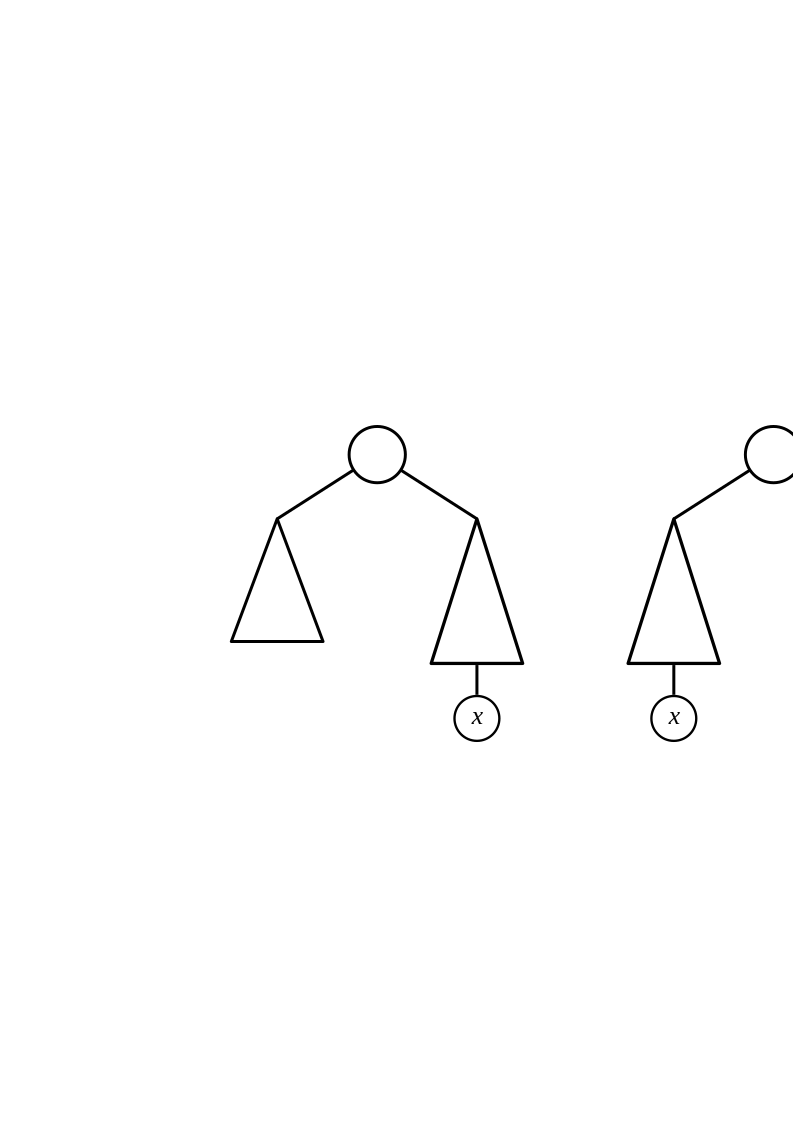
\includegraphics[scale=0.7]{Images/avl_insert_out_of_balance.png}
    \caption{Inserting makes AVL tree out of balance}
    \label{fig:oob_avl_tree}
\end{figure}

Even within this there are 2 (unfortunately asymmetric) cases to consider. But first we need more names: let $m$ be the `lowest ancestor' (i.e. with the ancestor with the greatest depth) of $x$ that is no longer AVL-balanced after the insertion of $x$. As we will see it suffices to fix the subtree rooted at $m$, so we will assume $m$ to be the root. Let $T_1$ be the left subtree of $m$, let $m_R$ be $m$'s right child with left and right subtrees $T_2$ and $T_3$ respectively. Suppose $T_1$ is of height $h$. We assumed $T$ to be right heavy implying that $m$'s right subtree (i.e. the tree rooted at $m_R$) is of height $h + 1$. 

Our first claim is the following.
\begin{lemma}
    $T_2$ and $T_3$ are both of the same height and in particular are of height $h$.
\end{lemma}
\begin{proof}
    We know that before the insertion of $x$, the balance factor of $m$ was 1 (recall we are assuming that we insert into the right subtree of a right heavy tree). Since the height of $m$'s left subtree was $h$, the height of its right subtree must be $h + 1$. This means that at least one of $m_R$'s subtrees, i.e. one of $T_2$ and $T_3$, is of height $h$. Without loss of generality we can assume it to be $T_2$ (this is one of those symmetric cases). Suppose $T_3$ is not of height $h$, then it must be of height $h - 1$ (by the AVL property we know the only possible heights for $T_3$ are $h, h + 1$ and $h - 1$. We assume it is not $h$ and if it was of height $h + 1$ then the tree rooted at $m$ would not have been AVL at the beginning). Since the insertion of $x$, knocks $m$ out of balance, we know it must be inserted in to $T_2$ (if it was inserted into $T_3$, $BF(m_R)$ would remain unchanged). This causes the height of $T_2$ to increase to $h + 1$ (if this height did not change then $BF(m_R)$ would again remain unchanged). But then $m_R$ is out of balance since its balance factor is now $(h - 1) - (h + 1) = -2$. However we assumed that $m$ was the lowest ancestor to be knocked out of balance, leading to a contradiction.
\end{proof}

Now that we have that sorted (ha!), we need to consider how to correct the tree after inserting $x$. As mentioned we split this into two cases, inserting into $T_2$ and inserting into $T_3$. The simpler case is inserting into $T_3$ so let us start with that. In this case, we can fix the tree with what's called a \textit{single (left) rotation} (if we were inserting into the left subtree of $m$'s left child we would do a single right rotation instead). This is most easily illustrated via diagrams. 

\begin{figure}[h]
    \centering
    \includegraphics[scale=0.6]{Images/avl_single_rotations.png}
    \caption{AVL (single) rotations}
    \label{fig:avl-sing-rotation}
\end{figure}

There are some important properties that the single rotation has:
\begin{minitemize}
    \item The tree rooted at $m$ is now balanced
    \item The BST property is maintined
    \item The rotation takes constant time (in fact only 3 pointers are changed)
    \item The height of the tree (rooted at $m$) is the same after the insertion + rotation as it was before the insertion
\end{minitemize}
The last one is a particularly important property. It means that after we have performed a single rotation to fix the balance, the rest of tree (above $m$) is also balanced now. Thus no more work needs to be done!

There is, however, work needing to be done for finishing the remainder of the algorithm. The only case that remains to be considered is if we insert $x$ into $T_2$. In this case (as you can check) a single rotation is not enough to fix the problem. However, if we stare long and hard, we might realise that performing a single right rotation on $m_R$ gets us to the previous case (where the insertion was on the right subtree of the right child of $m$). Therefore, to fix this case, we first rotate right on $m_R$ (to get a right-right heavy tree) and then rotate left on $m$ to get a balanced tree. This is called a \textit{double rotation}, with this specific process being called a double right left rotation (if we had inserted into $m_L$'s right subtree we would do a double left right rotation instead). Note that double rotations share the same properties that single rotations do (admitted a few more pointers need to changed but the operation remains constant time).

% TODO: Add diagram of double right left rotation

Let us then see what this algorithm looks like.

\begin{lstlisting}[language=, numberstyle=\color{white}]
INSERT(T, x):
Insert x into T as you would in a BST

Set BF of x to 0 and retrace path from x to root. For every node m:
i) if x was in m's right subtree, increment BF(m) by 1, if x was in m's left subtree, decrement BF(m) by 1.
ii) If BF(m) == 1 or BF(m) == -1, continue
iii) If BF(m) == 0, stop (an unbalanced tree is now balanced, no change needs to be made to ancestors)
iv) If BF(m) == 2 and BF(m_R) == 1, do a left rotation on m and stop
v) If BF(m) == 2 and BF(m_R) == -1, do a double right left rotation on m and stop
vi) If BF(m) == -2 and BF(m_L) == 1, do a double left right rotation on m and stop
vii) If BF(m) == -2 and BF(m_L) == -1, do a single right rotation on m and stop
viii) If m is the root, stop
\end{lstlisting}

\subsection{Delete}
The first thing to note with delete is that all cases boil down to deleting a leaf. Recall that there are 3 cases to consider when deleting from a BST: deleting a node with 0 children (i.e. a leaf), deleting a node with 1 child and deleting a node with 2 children. The first case remains the same. For the second case, with AVL trees, this necessitates that the sole child of the node is a leaf (otherwise we would be out of AVL balance). Thus we way swap this node with its child and then delete the leaf. For the last case, we swap the node with its successor, which is either a leaf or has one (right) child, getting us to previous cases in either case. Thus we only consider the case of deleting a leaf. For the remainder of this (sub)section any deletion can be assume to be of a leaf.

Once again there are two symmetric cases that cause an imbalance: deleting from the left subtree of a right heavy tree or deleting from the right subtree of a left heavy tree. As before we will only consider one case, the former one. The setup is the same as before: $m$ is the lowest ancestor of $x$ that is now out of balance. We denote its right subtree $T_3$ and it's left child $m_L$. The left and right subtrees at $m_L$ are called $T_1$ and $T_2$ respectively. We will again assume $T_3$ to be of height $h$ after the deletion of $x$ (so the height of $m$'s right subtree would have been $h + 1$ before deletion). Since $m$ is now too left heavy, we know its balance factor is $-2$. This means that the height of $m$'s left subtree is $h + 2$ hence at least one of $T_1$ and $T_2$ is of height $h + 1$. Let us first consider the case with $T_1$ being of height $h + 1$ (and $T_2$ can be of height $h$ or height $h + 1$). See \autoref{fig:avl-delete-case1} for the diagram. In this case we see that a single right rotation on $m$ rebalances the tree. One important thing to note, however, is that if $T_2$ is of height $h$, the height of tree after the rotation is \textit{is not the same as it was before deletion} but has been decremented by 1. We will return to this point later. For now we deal with the case where $T_1$ is of height $h$.

\begin{figure}[h]
    \centering
    \includegraphics[scale=0.5]{Images/avl_delete_case1.png}
    \caption{AVL Deletion case 1}
    \label{fig:avl-delete-case1}
\end{figure}

In the other case (with $T_2$ being of height $h + 1$ and $T_1$ of height $h$), as one might guess, we will need a double rotation (specifically a left right rotation). This being a bit more delicate operation, we should provide some more details. So first, names: let $m_{LR}$ be the right child of $m_L$ with left and right subtrees $T_{21}$ and $T_{22}$ respectively. Since we assume $T_2$ to be of height $h + 1$, we know that at least one of $T_{21}$ and $T_{22}$ is of height $h$. See \autoref{fig:avl-delete-case2} for the diagram. After the double rotation (a left rotation on $m_L$ followed by a right rotation on $m$), we see that $m_L$'s right child is now $T_{21}$ (the left child of course remains the same: $T_{1}$).
$m_{LR}$ is now at the root with $m$ as its right child ($m_L$ remains as the left child to the root). We see that $m$'s left child is now $T_{22}$ and the right child is now $T_3$. In particular this means that the height of $m_{LR}$'s left and right subtree (which remember is the root now) is $h + 1$ therefore the height of the tree rooted at $m_{LR}$ is $h + 2$. Since the tree was of height $h + 3$ before the deletion, in this scenario we are guaranteed to decrease the height of the tree.

\begin{figure}[h]
    \centering
    \includegraphics[scale=0.5]{Images/avl_delete_case2.png}
    \caption{AVL Deletion case 2}
    \label{fig:avl-delete-case2}
\end{figure}

The fact that trees may change height means that the balance factor of their parents may change and may cause these nodes higher up to be out of AVL balance. Thus after these rotations, we need to check that $m$'s parent is still in AVL balance and fix it via rotations again if not. How far do we need to continue this? If the height of the tree rooted at $m$ hasn't changed then we don't need to do anything of course. So suppose the height of $m$ has decreased. If $m$ was a left child, the balance factor of its parent increases by 1 and if it was a right child, the balance factor decreases by 1. If the parent $p$ was originally balanced then its going to be left or right heavy now but the height of tree rooted at $p$ has not changed ($m$'s sibling remains of the same height) therefore we don't need to do anything further up. If instead $BF(p)$ was originally $-1$ or 1 is now 0 then we've definitely made the tree shorter so we need check that the balance factor of its parent is fine. If the balance factor went from $-1/1$ to $-2/2$ then we do some rotations. If the tree is restored to its original height then no more works needs to be done. As usual though if the height has been shortened then we must check its parent and repeat the whole process. We summarise all this into the algorithm below.

In the worst case, we could end up making corrections all the way up to the root, totalling $O(\log n)$ rotations. Luckily with the rotations being constant time, this means this deletion algorithm is still $O(\log n)$. We end with the deletion algorithm written in full.

\begin{lstlisting}[language=, numberstyle=\color{white}]
DELETE(T, x):
Find node (leaf) x to delete

Trace the path back to the root. For every node m:
If BF(m) was previously 0:
    Update BF and exit. No further work needs to be done since the height of the tree rooted at m has not changed.
If BF(m) was previously -1 or 1 and is now 0:
    The tree rooted at m is now shorter. This may affect m's ancestors so we continue moving up the tree.
If BF(m) was previously -1 or 1 and is now -2 or 2:
    Perform the appropriate rotation. If the height of the tree rooted at m is the same, we can quit. If it has changed we continue moving up the tree
\end{lstlisting}

\subsection{Key Ideas}
There is often a competition that occurs between operations: optimising one operation to its maximal point often comes at the cost of making other operations more expensive (ideally we would like to maintain a perfect BST for above but this makes insertion and deletion too expensive). Hence we strike a compromise between these to make all operations relatively fast. This is a key (and as you can see recurring) idea when designing algorithms.

Another important note is that by storing extra information on existing data structures, we can improve those data structures (after all AVL trees are simply BSTs with the additional BF data!). This is known as augmenting data structures (see the following section). This lightly highlights another tension in computer science: we can often save on runtime by sacrificing space (i.e. memory) and vice versa. Our goal is to find an optimal balance between the two.